\documentclass[lettersize,journal]{IEEEtran}
\usepackage{amsmath,amsfonts}
\usepackage{algorithmic}
\usepackage{array}
\usepackage[caption=false,font=normalsize,labelfont=sf,textfont=sf]{subfig}
\usepackage{textcomp}
\usepackage{stfloats}
\usepackage{url}
\usepackage{verbatim}
\usepackage{graphicx}
\def\BibTeX{{\rm B\kern-.05em{\sc i\kern-.025em b}\kern-.08em
    T\kern-.1667em\lower.7ex\hbox{E}\kern-.125emX}}
\usepackage{balance}

\begin{document}
\title{Paris housing price prediction \\ {\small ~~~~~~~~~~~~~~~~~~~~~~~~~~~~~~~~  --- Python Data Analysis Course Paper} }
\author{Information Science and Engineering Department
\\Yihao Chen\\2020010787
}

\markboth{Petroleum Computer Science,~Vol.~18, No.~1, May~2023}%
{How to Use the IEEEtran \LaTeX \ Templates}

\maketitle

\begin{abstract}
%The abstract should be about 200 words long. DO NOT USE SPECIAL CHARACTERS, SYMBOLS, OR MATH IN YOUR TITLE OR ABSTRACT. 
%The prediction of house price increase in Paris is usually used to study, and the influencing factors related to it include housing area, construction date, whether some hardware amenities are perfect, etc. In this topic, it is influenced by 17-dimensional variables, and of course, there are more influencing factors worth exploring. In my previous research, the papers I researched mostly used traditional machine learning methods to accurately predict house prices, so I used methods such as Random Forest and XGboost to analyze the problem, and also did feature engineering processing on the given influencing factors to optimize our final prediction effect. At the same time, I compare and analyze these methods, investigate their differences, and make an evaluation as well as a conclusion of our model.
The prediction of house price increase in Paris is usually used to study, and the influencing factors related to it include housing area, construction date, whether some hardware amenities are perfect, etc. In this topic, it is influenced by 17-dimensional variables, and of course, there are more influencing factors worth exploring. In my previous research, the papers I researched mostly used traditional machine learning methods to accurately predict house prices, so I used methods such as Random Forest and XGboost to analyze the problem, and also did feature engineering processing on the given influencing factors to optimize our final prediction effect. At the same time, I compare and analyze these methods, investigate their differences, and make an evaluation as well as a conclusion of our model.
\end{abstract}

\begin{IEEEkeywords}
    
keyword1, keyword2, keyword3.
\end{IEEEkeywords}

%表格做法
\begin{table}
    \centering
    \begin{tabular}{l|r}
    Item & Quantity \\\hline
    Widgets & 42 \\
    Gadgets & 13
    \end{tabular}

\section{Introduction}
\IEEEPARstart{T}{his}  template provides students with most of the formatting specifications needed for preparing electronic versions of their papers. PLEASE DO NOT RE-ADJUST THESE MARGINS.

\section{Method}
\noindent Add the specific {\bf{method}} of your experiment here.

\section{Experiment}
\noindent Add your {\bf{experiment}} here.

\section{Conclusion}
\noindent Add your {\bf{conclusion}} here.

\section{How to Create Common Front Matter}
\noindent The following sections describe general coding for these common elements.
\subsection{Paper Title}
\noindent The title of your paper is coded as:

\begin{verbatim}
\title{The Title of Your Paper}
\end{verbatim}

\noindent Please try to avoid the use of math or chemical formulas in your title if possible.

\subsection{Abstracts}
\noindent The abstract is the first element of a paper after the $\backslash${\tt{maketitle}} macro is invoked.  The coding is simply:
\begin{verbatim}
\begin{abstract}
Text of your abstract.
\end{abstract}
\end{verbatim}
Please try to avoid mathematical and chemical formulas in the abstract.

\subsection{Index Terms}
\noindent The index terms are used to help other researchers discover your paper. Each society may have it's own keyword set. Contact the EIC of your intended publication for this list.
\begin{verbatim}
\begin{IEEEkeywords}
Broad band networks, quality of service
\end{IEEEkeywords}
\end{verbatim}
\section{How to Create Common Body Elements}
\noindent The following sections describe common body text elements and how to code them.

\subsection{Initial Drop Cap Letter}
\noindent The first text paragraph uses a ``drop cap'' followed by the first word in ALL CAPS. This is accomplished by using the $\backslash${\tt{IEEEPARstart}} command as follows:
\begin{verbatim}
\IEEEPARstart{T}{his} is the first paragraph 
of your paper. . .
\end{verbatim}

\subsection{Sections and Subsections}
\noindent Section headings use standard \LaTeX\ commands: $\backslash${\tt{section}}, $\backslash${\tt{subsection}} and $\backslash${\tt{subsubsection}}. Numbering is handled automatically for you and varies according to type of publication. It is common to not indent the first paragraph following a section head by using $\backslash${\tt{noindent}} as follows:
\begin{verbatim}
\section{Section Head}
\noindent The text of your paragraph . . .
\end{verbatim}

\subsection{Citations to the Bibliography}
\noindent The coding for the citations are made with the \LaTeX\ $\backslash${\tt{cite}} command. This will produce individual bracketed reference numbers in the IEEE style. At the top of your \LaTeX\ file you should include:
\begin{verbatim}
\usepackage{cite}
\end{verbatim}
For a single citation code as follows:
\begin{verbatim}
see \cite{ams}
\end{verbatim}
This will display as: see \cite{ams}\\

For multiple citations code as follows:
\begin{verbatim}
\cite{ams,oxford,lacomp}
\end{verbatim}

This will display as \cite{ams,oxford,lacomp}

\subsection{Figures}
\noindent Figures are coded with the standard \LaTeX\ commands as follows:
\begin{verbatim}
\begin{figure}[!t]
\centering
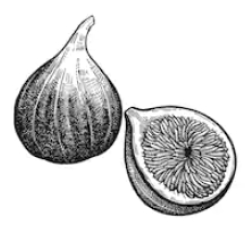
\includegraphics[width=2.5in]{fig1}
\caption{This is the caption for one fig.}
\label{fig1}
\end{figure}
\end{verbatim}
The [!t] argument enables floats to the top of the page to follow IEEE style. Make sure you include:
\begin{verbatim}
\usepackage{graphicx}
\end{verbatim}
 
\noindent at the top of your \LaTeX file with the other package declarations. 

To cross-reference your figures in the text use the following code example:
\begin{verbatim}
See figure \ref{fig1} ...
\end{verbatim}
This will produce:\\
See figure \ref{fig1} . . .

\begin{figure}[!t]
\centering
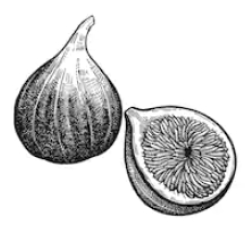
\includegraphics[width=2.5in]{fig1}
\caption{This is the caption for one fig.}
\label{fig1}
\end{figure}

\subsection{Tables}
\noindent Tables should be coded with the standard \LaTeX\ coding. The following example shows a simple table.


\begin{verbatim}
\begin{table}
\begin{center}
\caption{Filter design equations  ...}
\label{tab1}
\begin{tabular}{| c | c | c |}
\hline
Order & Arbitrary coefficients & 
coefficients\\
of filter & $e_m$ &   $b_{ij}$ \\
\hline
1& $b_{ij}=\hat{e}.\hat{\beta_{ij}}$, 
& $b_{00}=0$\\
\hline
2&$\beta_{22}=(~1,-1,-1,~~1,~~1,~~1)$ &\\ 
\hline
3& $b_{ij}=\hat{e}.\hat{\beta_{ij}}$, 
& $b_{00}=0$,\\
\hline 
\end{tabular}
\end{center}
\end{table}
\end{verbatim}
To reference the table in the text, code as follows:
\begin{verbatim}Table~\ref{tab1} lists the closed-form...\end{verbatim}

%moved here for pagination purposes
\begin{table}
\begin{center}
\caption{A Simple Table Example.}
\label{tab1}
\begin{tabular}{| c | c | c |}
\hline
Order & Arbitrary coefficients & coefficients\\
of filter & $e_m$ &   $b_{ij}$ \\
\hline
1& $b_{ij}=\hat{e}.\hat{\beta_{ij}}$, & $b_{00}=0$\\
\hline
2&$\beta_{22}=(~1,-1,-1,~~1,~~1,~~1)$ &\\ 
\hline
3& $b_{ij}=\hat{e}.\hat{\beta_{ij}}$, & $b_{00}=0$,\\
\hline 
\end{tabular}
\end{center}
\end{table}

\section{How to Create Common Back Matter Elements}
\noindent The following sections demonstrate common back matter elements such as Acknowledgments, Bibliographies, Appendicies and Author Biographies.

\subsection{Acknowledgments}
\noindent This should be a simple paragraph before the bibliography to thank those individuals and institutions who have supported your work on this article.

\begin{verbatim}
\section{Acknowledgments}
\noindent Text describing those who 
supported your paper.
\end{verbatim}

\subsection{Bibliographies}
\noindent {\bf{References Simplified:}} A simple way of composing references is to use the $\backslash${\tt{bibitem}} macro to define the beginning of a reference as in the following examples:\\


\noindent [6] H. Sira-Ramirez. ``On the sliding mode control of nonlinear systems,'' \textit{Systems \& Control Letters}, vol. 19, pp. 303--312, 1992.

\noindent coded as:
\begin{verbatim}
\bibitem{Sira3}
H. Sira-Ramirez. ``On the sliding mode 
control of nonlinear systems,'' 
\textit{Systems \& Control Letters}, 
vol. 19, pp. 303--312, 1992.
\end{verbatim}

\subsection{Biographies and Author Photos}
\noindent Authors may have options to include their photo or not. Photos should be a bit-map graphic (.tif or .jpg) and sized to fit in the space allowed. Please see the coding samples below:
\begin{verbatim}
\begin{IEEEbiographynophoto}{Jane Doe}
Biography text here without a photo.
\end{IEEEbiographynophoto}
\end{verbatim}
or a biography with a photo

\begin{verbatim}
\begin{IEEEbiography}[{
\includegraphics
[width=1in,height=1.25in,clip,
keepaspectratio]{fig2.png}}]
{Information Science and Engineering Department} 
In this paragraph you can place 
your educational, professional background 
and research and other interests.
\end{IEEEbiography}
\end{verbatim}

\begin{thebibliography}{1}

\bibitem{ams}
{\it{Mathematics into Type}}, American Mathematical Society. Online available: 

\bibitem{oxford}
T.W. Chaundy, P.R. Barrett and C. Batey, {\it{The Printing of Mathematics}}, Oxford University Press. London, 1954.

\bibitem{lacomp}{\it{The \LaTeX Companion}}, by F. Mittelbach and M. Goossens

\bibitem{mmt}{\it{More Math into LaTeX}}, by G. Gr\"atzer

\bibitem{amstyle}{\it{AMS-StyleGuide-online.pdf,}} published by the American Mathematical Society

\bibitem{Sira3}
H. Sira-Ramirez. ``On the sliding mode control of nonlinear systems,'' \textit{Systems \& Control Letters}, vol. 19, pp. 303--312, 1992.

\bibitem{Levant}
A. Levant. ``Exact differentiation of signals with unbounded higher derivatives,''  in \textit{Proceedings of the 45th IEEE Conference on Decision and Control}, San Diego, California, USA, pp. 5585--5590, 2006.

\bibitem{Cedric}
M. Fliess, C. Join, and H. Sira-Ramirez. ``Non-linear estimation is easy,'' \textit{International Journal of Modelling, Identification and Control}, vol. 4, no. 1, pp. 12--27, 2008.

\bibitem{Ortega}
R. Ortega, A. Astolfi, G. Bastin, and H. Rodriguez. ``Stabilization of food-chain systems using a port-controlled Hamiltonian description,'' in \textit{Proceedings of the American Control Conference}, Chicago, Illinois, USA, pp. 2245--2249, 2000.

\end{thebibliography}

\begin{IEEEbiography}[{
\includegraphics[width=1in,height=1.25in,clip,keepaspectratio]{fig2.png}}]{Information Science and Engineering Department}
In this paragraph you can place your educational, professional background and research and other interests.\end{IEEEbiography}


\end{document}


